A 2-axis sun tracking mechanism is illustrated in \refFig{fig:tilted-surface-sun-tracking}. An optimal angle configurations exists so that a \ac{SA} surface generates the maximum amount of power for a given period. These angles are the $\gamma_{c}$ orientation angle (surface azimuth angle) and the $\beta$ inclination angle.

\begin{figure}[h]
  \centering
  \hypersetup{linkcolor=captionTextColor}
  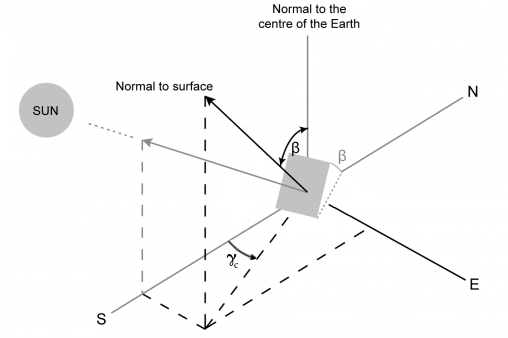
\includegraphics[width=0.7\linewidth]{sections/appendix/optimal-angles/images/beta-and-gamma-angles-on-tilted-surface.png}\\
  \caption[Solar array surface inclination and orientation]
          {\ac{SA} surface inclination and orientation. $\theta$ is the Sun angle of incidence. $\beta$ is the inclination angle and $\gamma_{c}$ is the orientation angle (i.e. the surface azimuth angle). $\gamma_{c} = \SI{0}{\degree}$ when facing the equator, negative when facing East ($\gamma_{c} = \SI{-90}{\degree}$), and positive when facing West ($\gamma_{c} = \SI{+90}{\degree}$). Image taken from \citeother{ITACA} and modified for this study.}
  \label{fig:tilted-surface-sun-tracking}
\end{figure}

\section{Optimal Angles}
For clear skies, two approaches to determine the optimal angles for $\gamma_{c}$ and $\beta$ are presented in \citemarsenv{Appelbaum1993}. \refEqn{eq:optimal_beta_irradiance} is described as a ``coarse approximation'' in \citeother{Soulayman2016} and gives an optimal $\beta$ based on the direct beam irradiance at noon:

\begin{equation}
  \label{eq:optimal_beta_irradiance}
  \beta_{p} = \phi - \delta_{p}
\end{equation}

where $\beta_{p}$ is the optimal inclination angle for a period $p$, $\phi$ is the planetary latitude, and $\delta_{p}$ is the average declination angle for the period $p$. A ``better approximation'' is shown in \citemarsenv{Appelbaum1995} based on the daily beam insolation on the surface from sunrise to sunset. However, comparing the results using this method to those obtained with \refEqn{eq:optimal_beta_irradiance} suggest a sign error in the published formula which has been rectified in \refEqn{eq:optimal_tanbeta_insolation}.

\begin{equation}
  \label{eq:optimal_tanbeta_insolation}
  \tan{(\beta)} = -\frac{\cos{(\omega_{sr})}\sin{(\phi)}\cos{(\delta)}-\left[1-\left(\frac{2\omega_{sr}}{\pi}\right)^{2}\right]\cos{(\phi)}\sin{(\delta)}}{\cos{(\omega_{sr})}\cos{(\phi)}\cos{(\delta)}+\left[1+\left(\frac{2\omega_{sr}}{\pi}\right)^{2}\right]\sin{(\phi)}\sin{(\delta)}}
\end{equation}


where $\omega_{sr}$ is the sunrise hour angle. The sign error correction is not necessary for $L_{s} = \SI{180}{\degree}$, as shown in \refEqn{eq:optimal_tanbeta_insolation_Ls180}.

\begin{equation}
  \label{eq:optimal_tanbeta_insolation_Ls180}
  \tan{(\beta_{L_{s} = \SI{180}{\degree}})} = \frac{\cos{(\omega_{sr})}\sin{(\phi)}\cos{(\delta)}-\left[1-\left(\frac{2\omega_{sr}}{\pi}\right)^{2}\right]\cos{(\phi)}\sin{(\delta)}}{\cos{(\omega_{sr})}\cos{(\phi)}\cos{(\delta)}+\left[1+\left(\frac{2\omega_{sr}}{\pi}\right)^{2}\right]\sin{(\phi)}\sin{(\delta)}}
\end{equation}

Facing the equator implies a direct orientation towards the sun thus the optimal value for $\gamma_{c}$ is widely accepted as being $\SI{0}{\degree}$. However, plotting out predicted insolations for all orientations at $\SI{1}{\degree}$ increments suggests otherwise, as is shown in \refSec{sec:Appendix:OptimalAngles:IaniChaos} and \refSec{sec:Appendix:OptimalAngles:IsmeniusCavus}.

\section{Iani Chaos}
\label{sec:Appendix:OptimalAngles:IaniChaos}

\refFig{fig:plot:optimal-angles-iani-chaos} plots daily insolations throughout a Martian year at Iani Chaos for $\beta_{opt}$ angles with different $\gamma_{c}$ orientations. Daily insolations on a flat surface are also included as a reference. An equator facing (North) orientation is suggested only during the first half of the Martian year, after which a northwestern facing orientation becomes more optimal.

\begin{figure}[h]
\captionsetup[subfigure]{justification=centering}
\vspace{-2ex}
\centering
    %% setup sizes
    \setlength{\subfigureWidth}{0.50\textwidth}
    \setlength{\graphicsHeight}{80mm}
    %% kill hyper-link highlighting
    \hypersetup{hidelinks=true}%
    %% the figures
    \begin{subfigure}[t]{\subfigureWidth}
        \centering
            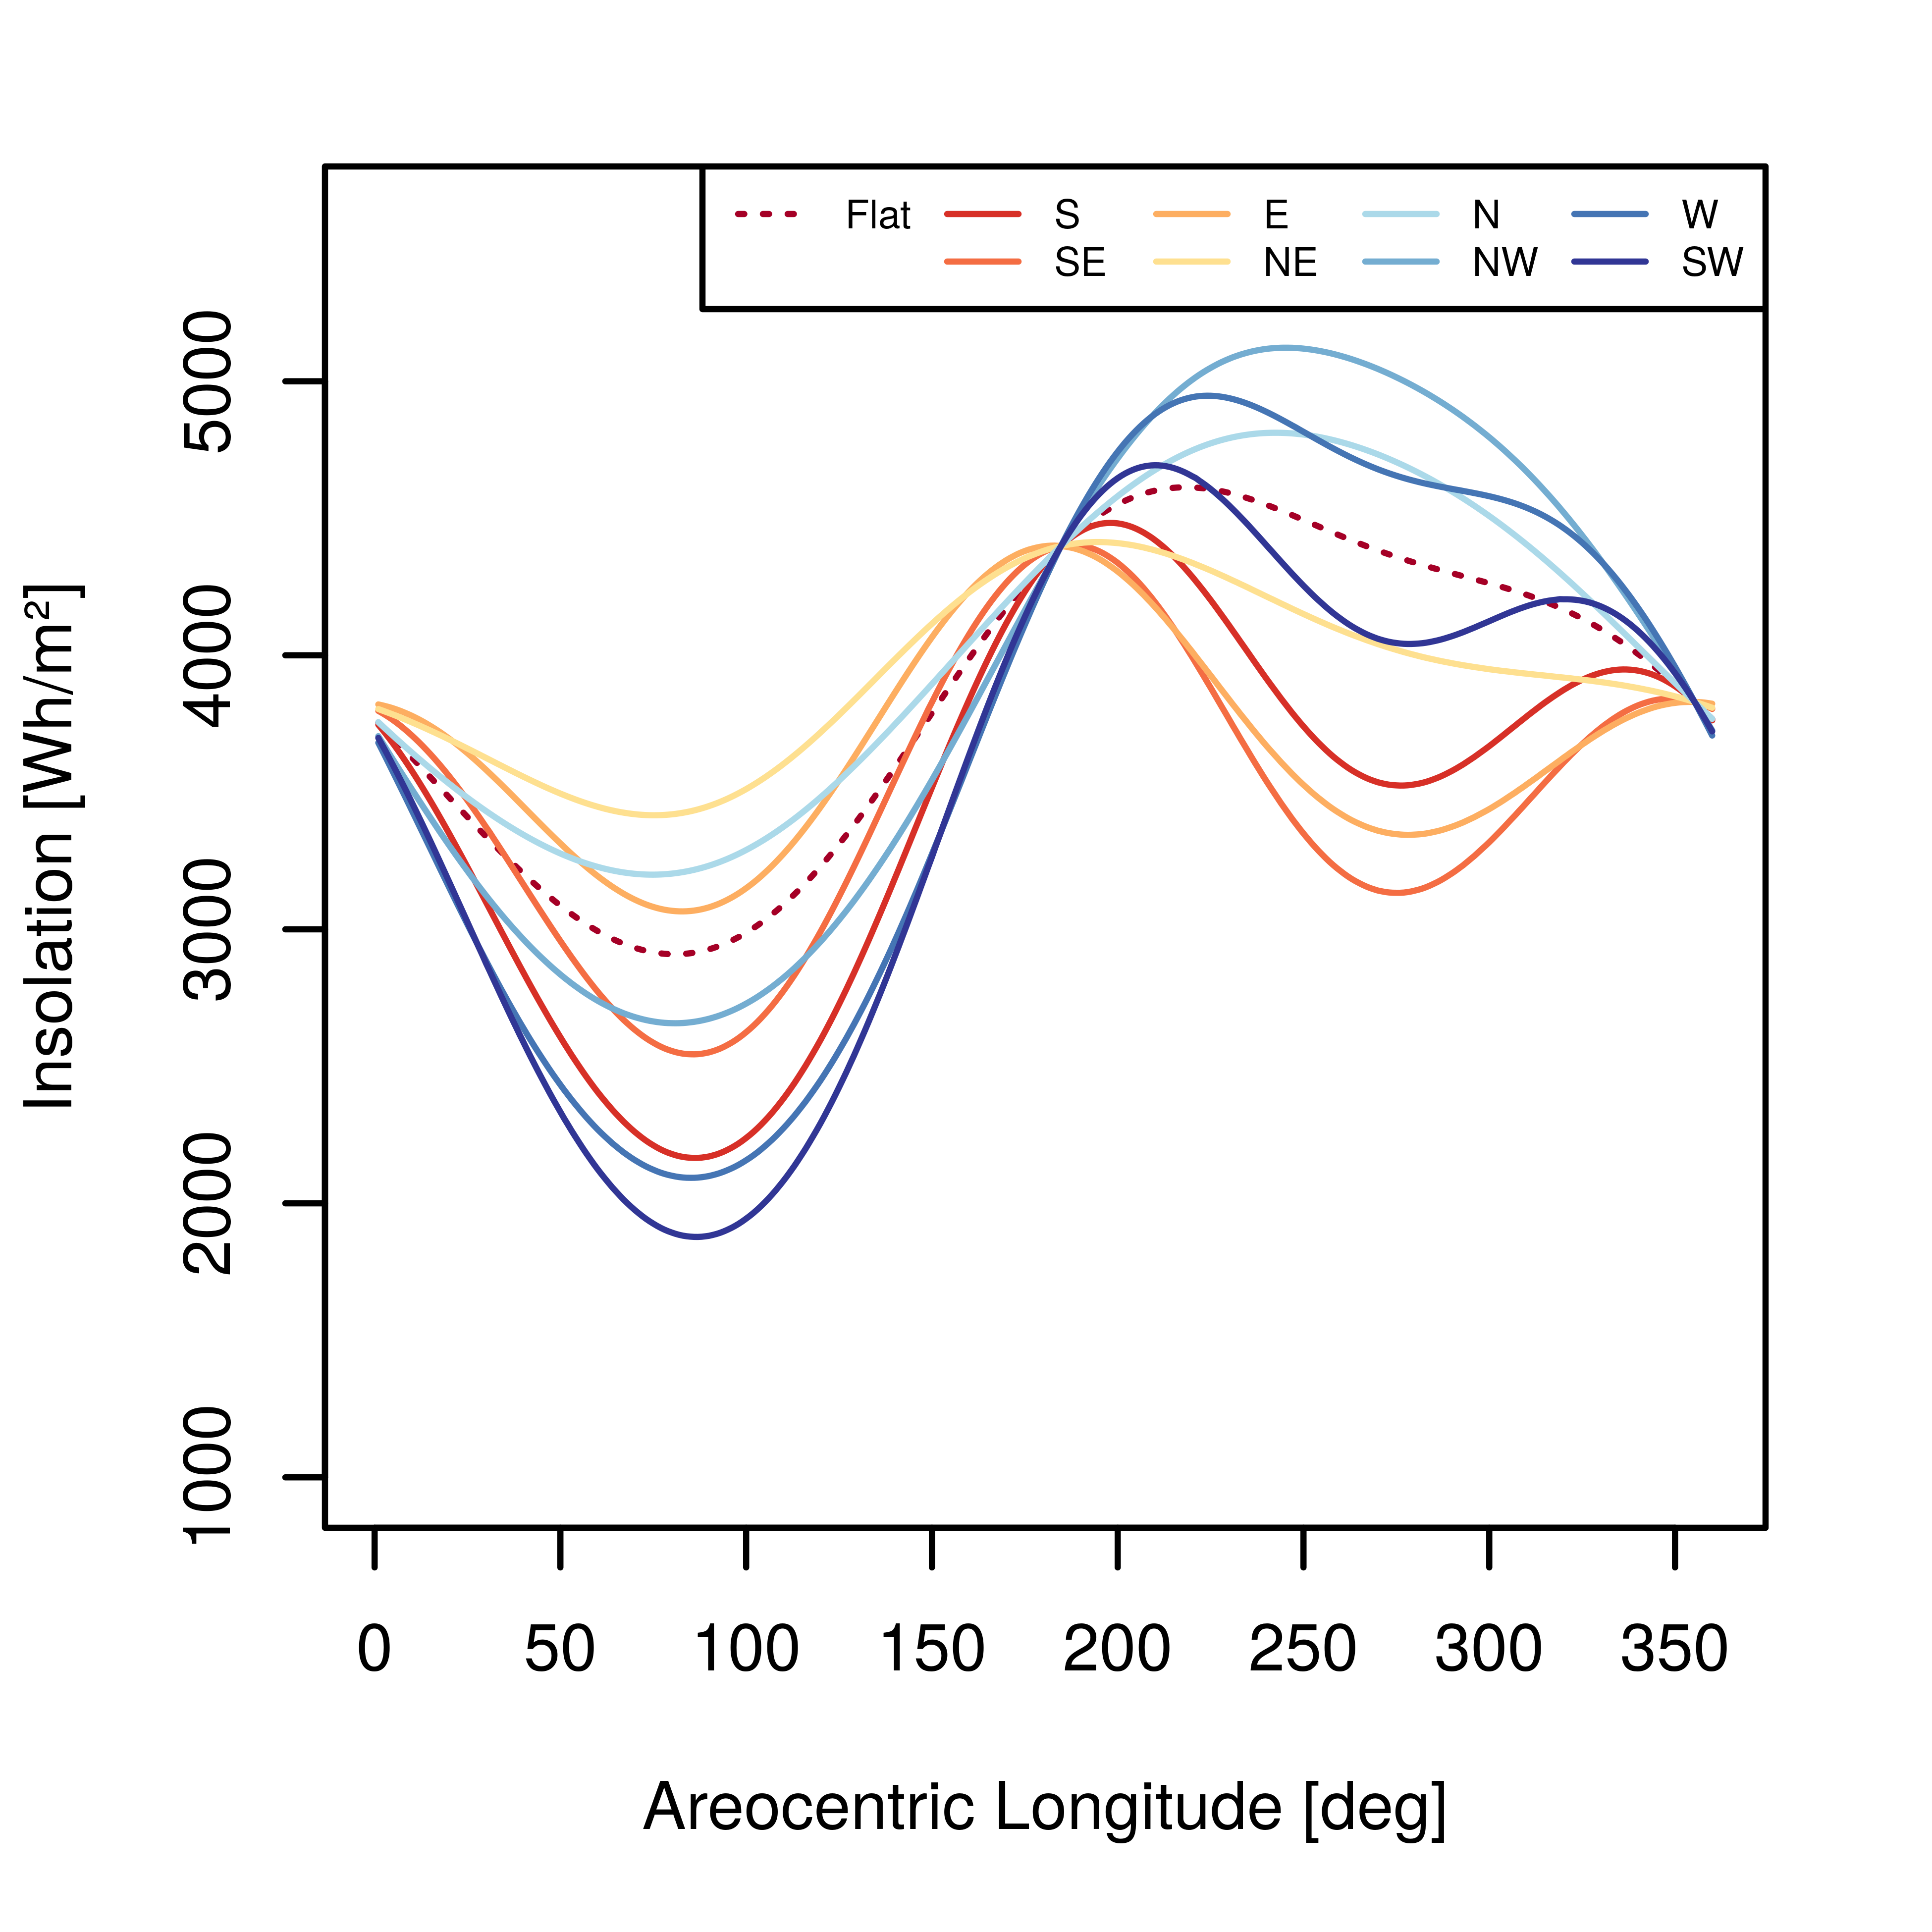
\includegraphics[height=\graphicsHeight]{sections/appendix/optimal-angles/plots/iani-chaos-tau-04-and-beta-optimal-based-on-direct-beam-irradiance-at-noon.png}
            \subcaption{Based on the direct beam irradiance at noon}
            \label{fig:sub:optimal-angles-iani-chaos-based-on-irradiance}
    \end{subfigure}\hfill
    \begin{subfigure}[t]{\subfigureWidth}
        \centering
            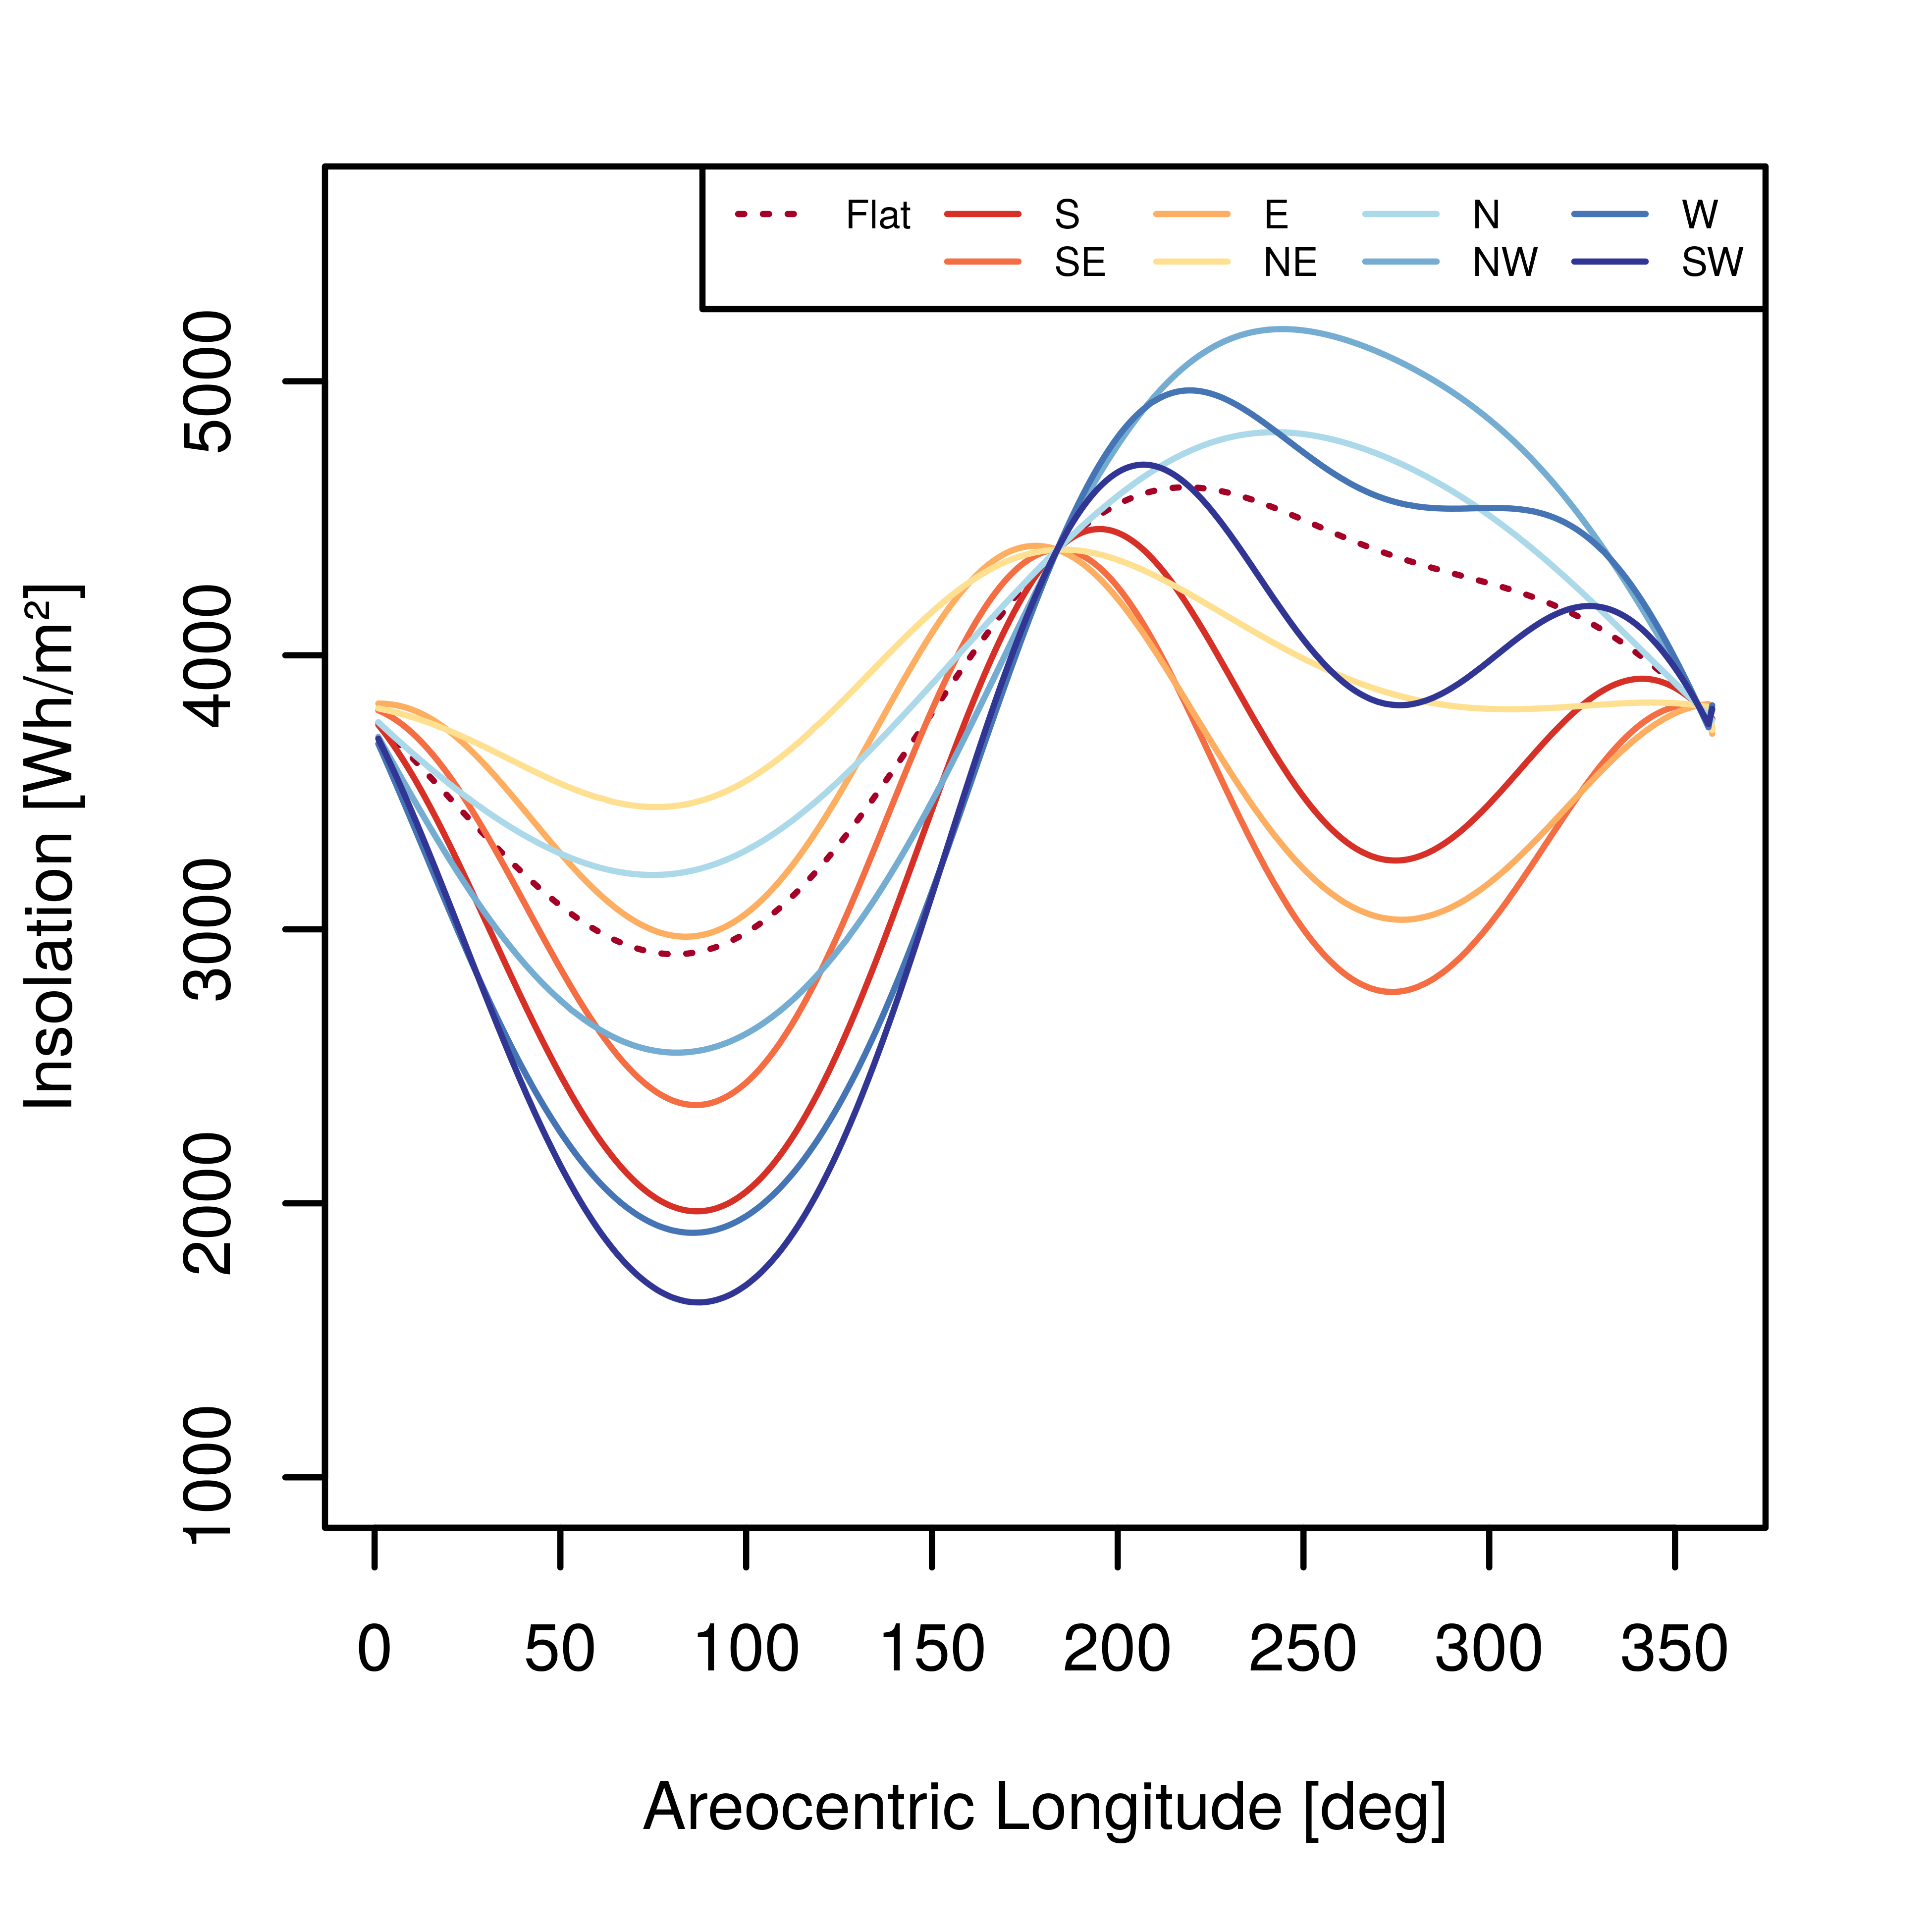
\includegraphics[height=\graphicsHeight]{sections/appendix/optimal-angles/plots/iani-chaos-tau-04-and-beta-optimal-based-on-solar-insolation.png}
            \subcaption{Based on the daily beam insolation on the surface from sunrise to sunset}
            \label{fig:sub:optimal-angles-iani-chaos-based-on-insolation}
    \end{subfigure}\\[0.8ex]
    \caption[Daily insolation at Iani Chaos for optimal inclinations with different orientations]
    {Daily insolation at Iani Chaos for optimal inclinations with different orientations. Clear day at $\tau=0.4$. Iani Chaos is located in the Sourthern hemisphere at latitude \SI{2}{\degree}S.}
    \label{fig:plot:optimal-angles-iani-chaos}
\vspace{-2ex}
\end{figure}

\section{Ismenius Cavus}
\label{sec:Appendix:OptimalAngles:IsmeniusCavus}

\refFig{fig:plot:optimal-angles-ismenius-cavus} plots daily insolations throughout a Martian year at Ismenius Cavus for $\beta_{opt}$ angles with different $\gamma_{c}$ orientations. Daily insolations on a flat surface are also included as a reference. Throughout the entire year, a southwestern orientation appears more optimal than South facing.

\begin{figure}[h]
\captionsetup[subfigure]{justification=centering}
\vspace{-2ex}
\centering
    %% setup sizes
    \setlength{\subfigureWidth}{0.50\textwidth}
    \setlength{\graphicsHeight}{80mm}
    %% kill hyper-link highlighting
    \hypersetup{hidelinks=true}%
    %% the figures
    \begin{subfigure}[t]{\subfigureWidth}
        \centering
            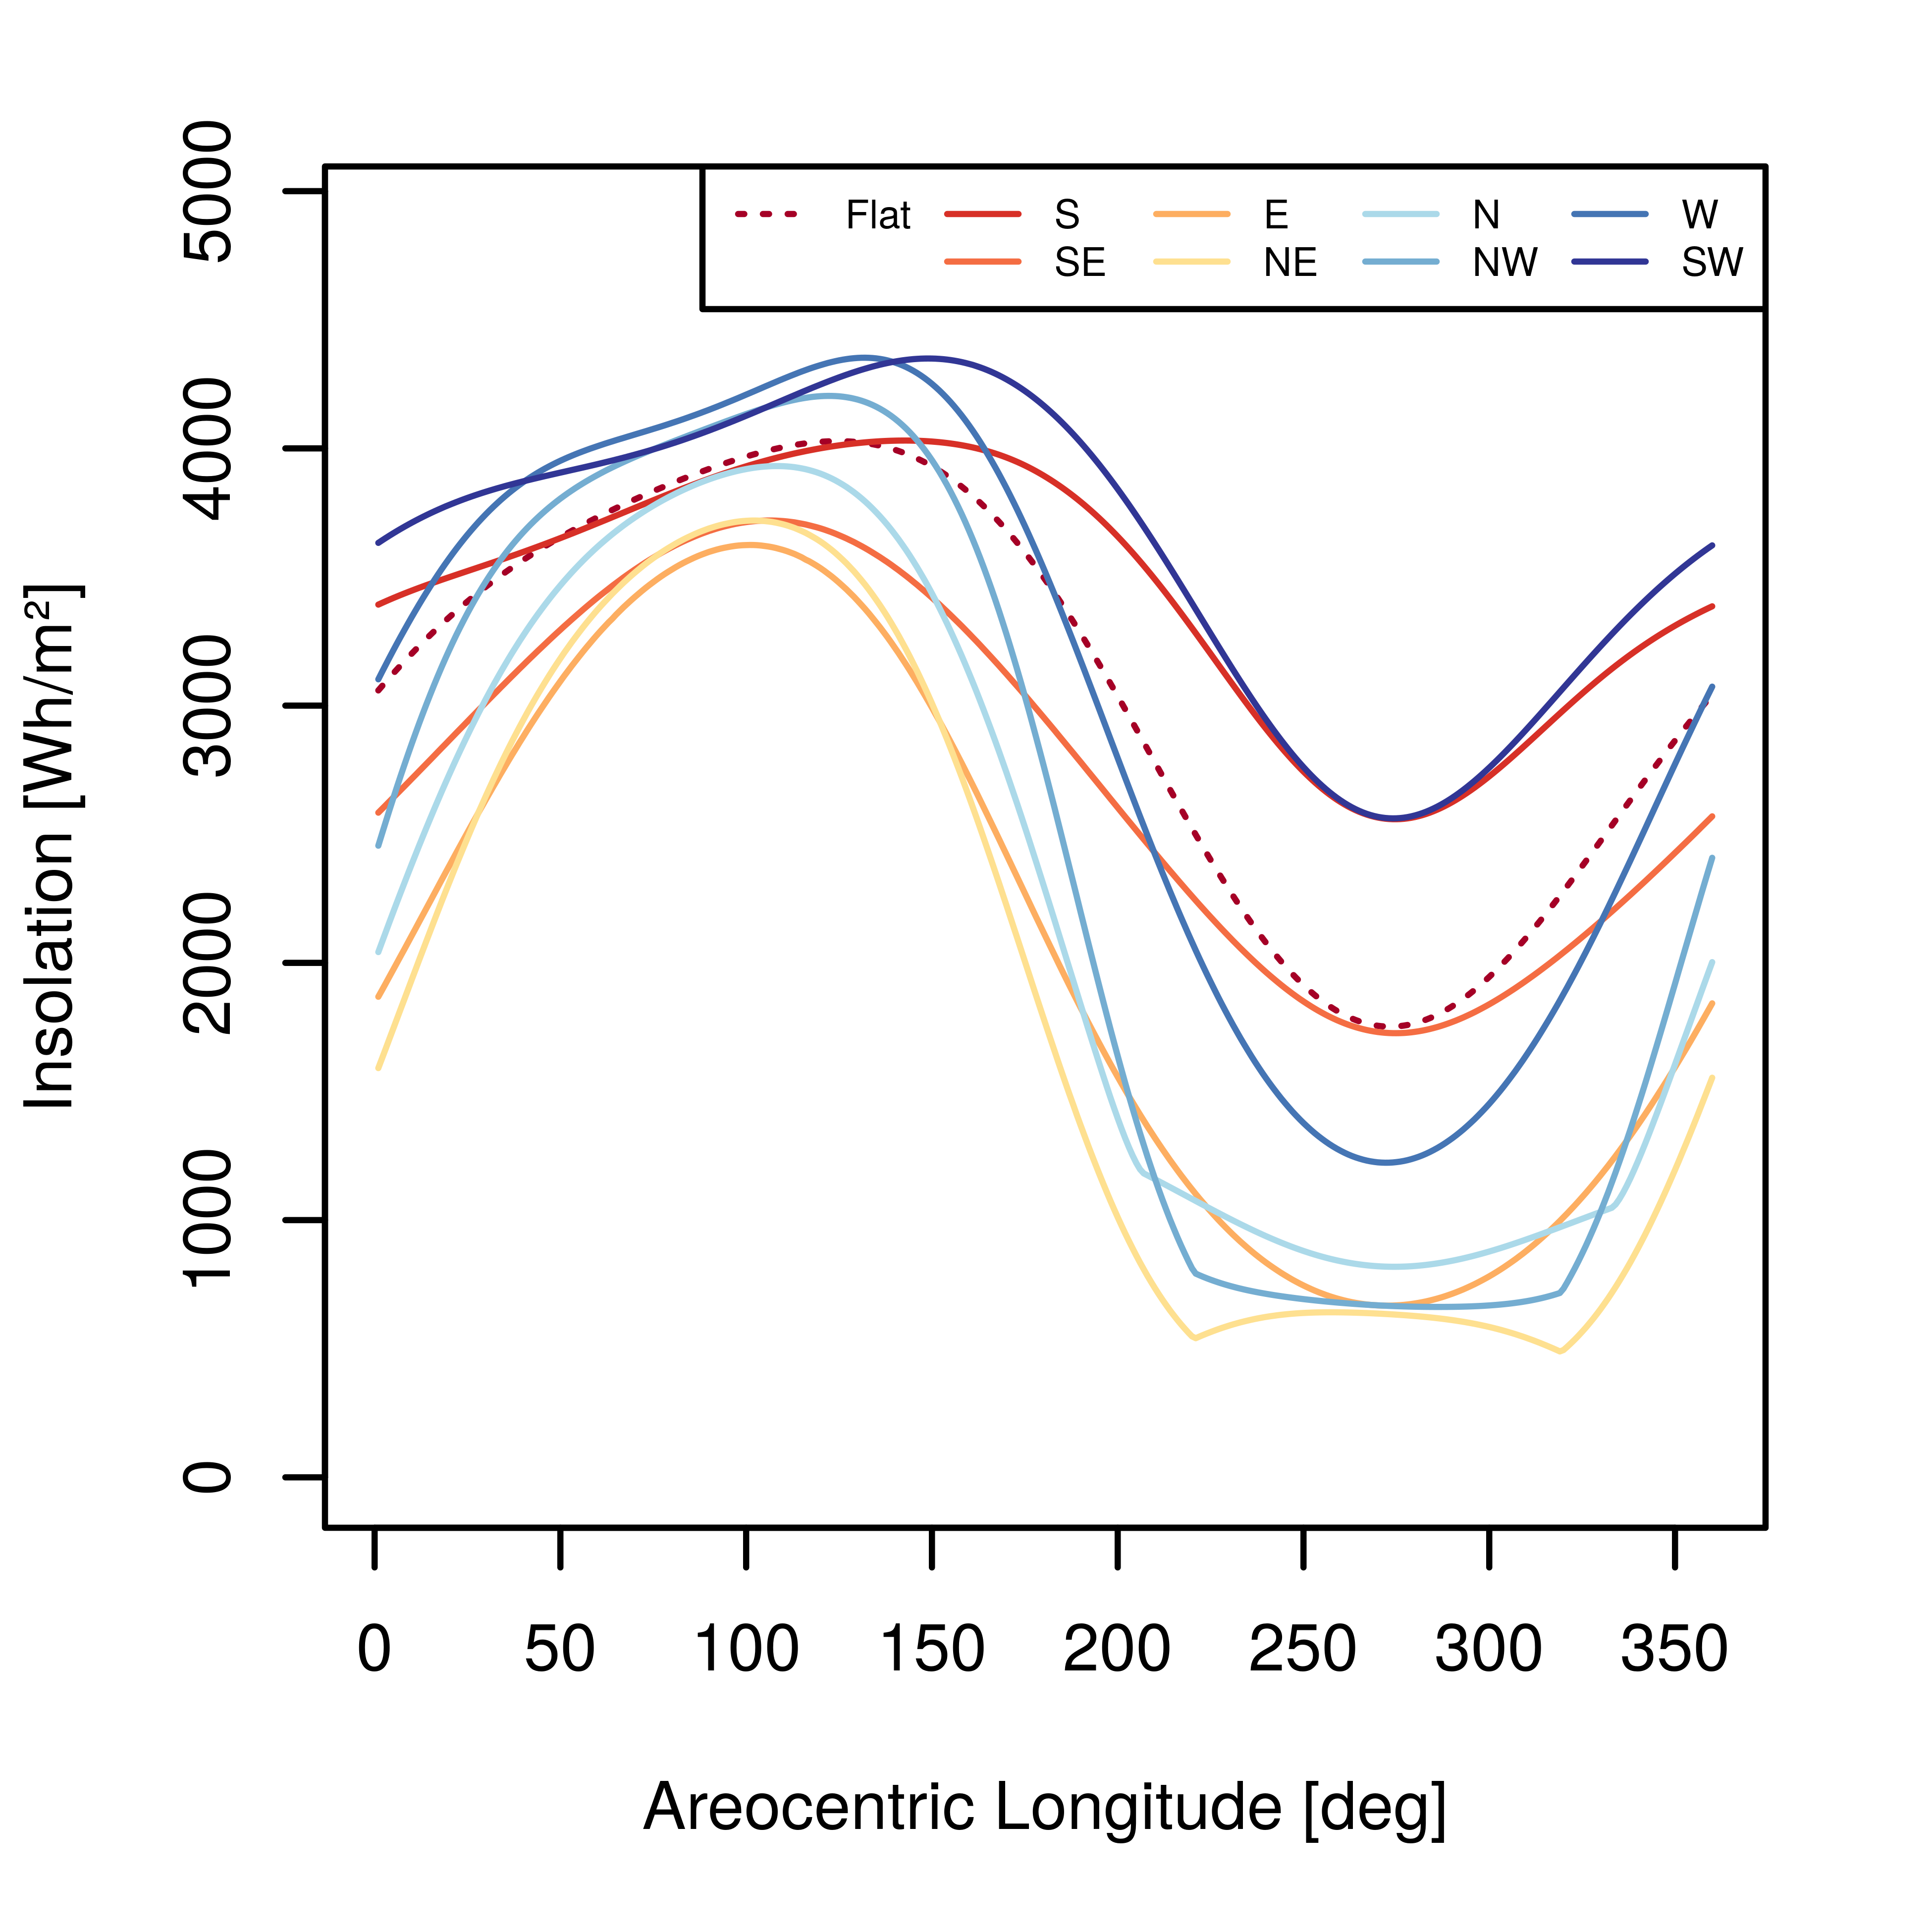
\includegraphics[height=\graphicsHeight]{sections/appendix/optimal-angles/plots/ismenius-cavus-tau-04-and-beta-optimal-based-on-direct-beam-irradiance-at-noon.png}
            \subcaption{Based on the direct beam irradiance at noon}
            \label{fig:sub:optimal-angles-ismenius-cavus-based-on-irradiance}
    \end{subfigure}\hfill
    \begin{subfigure}[t]{\subfigureWidth}
        \centering
            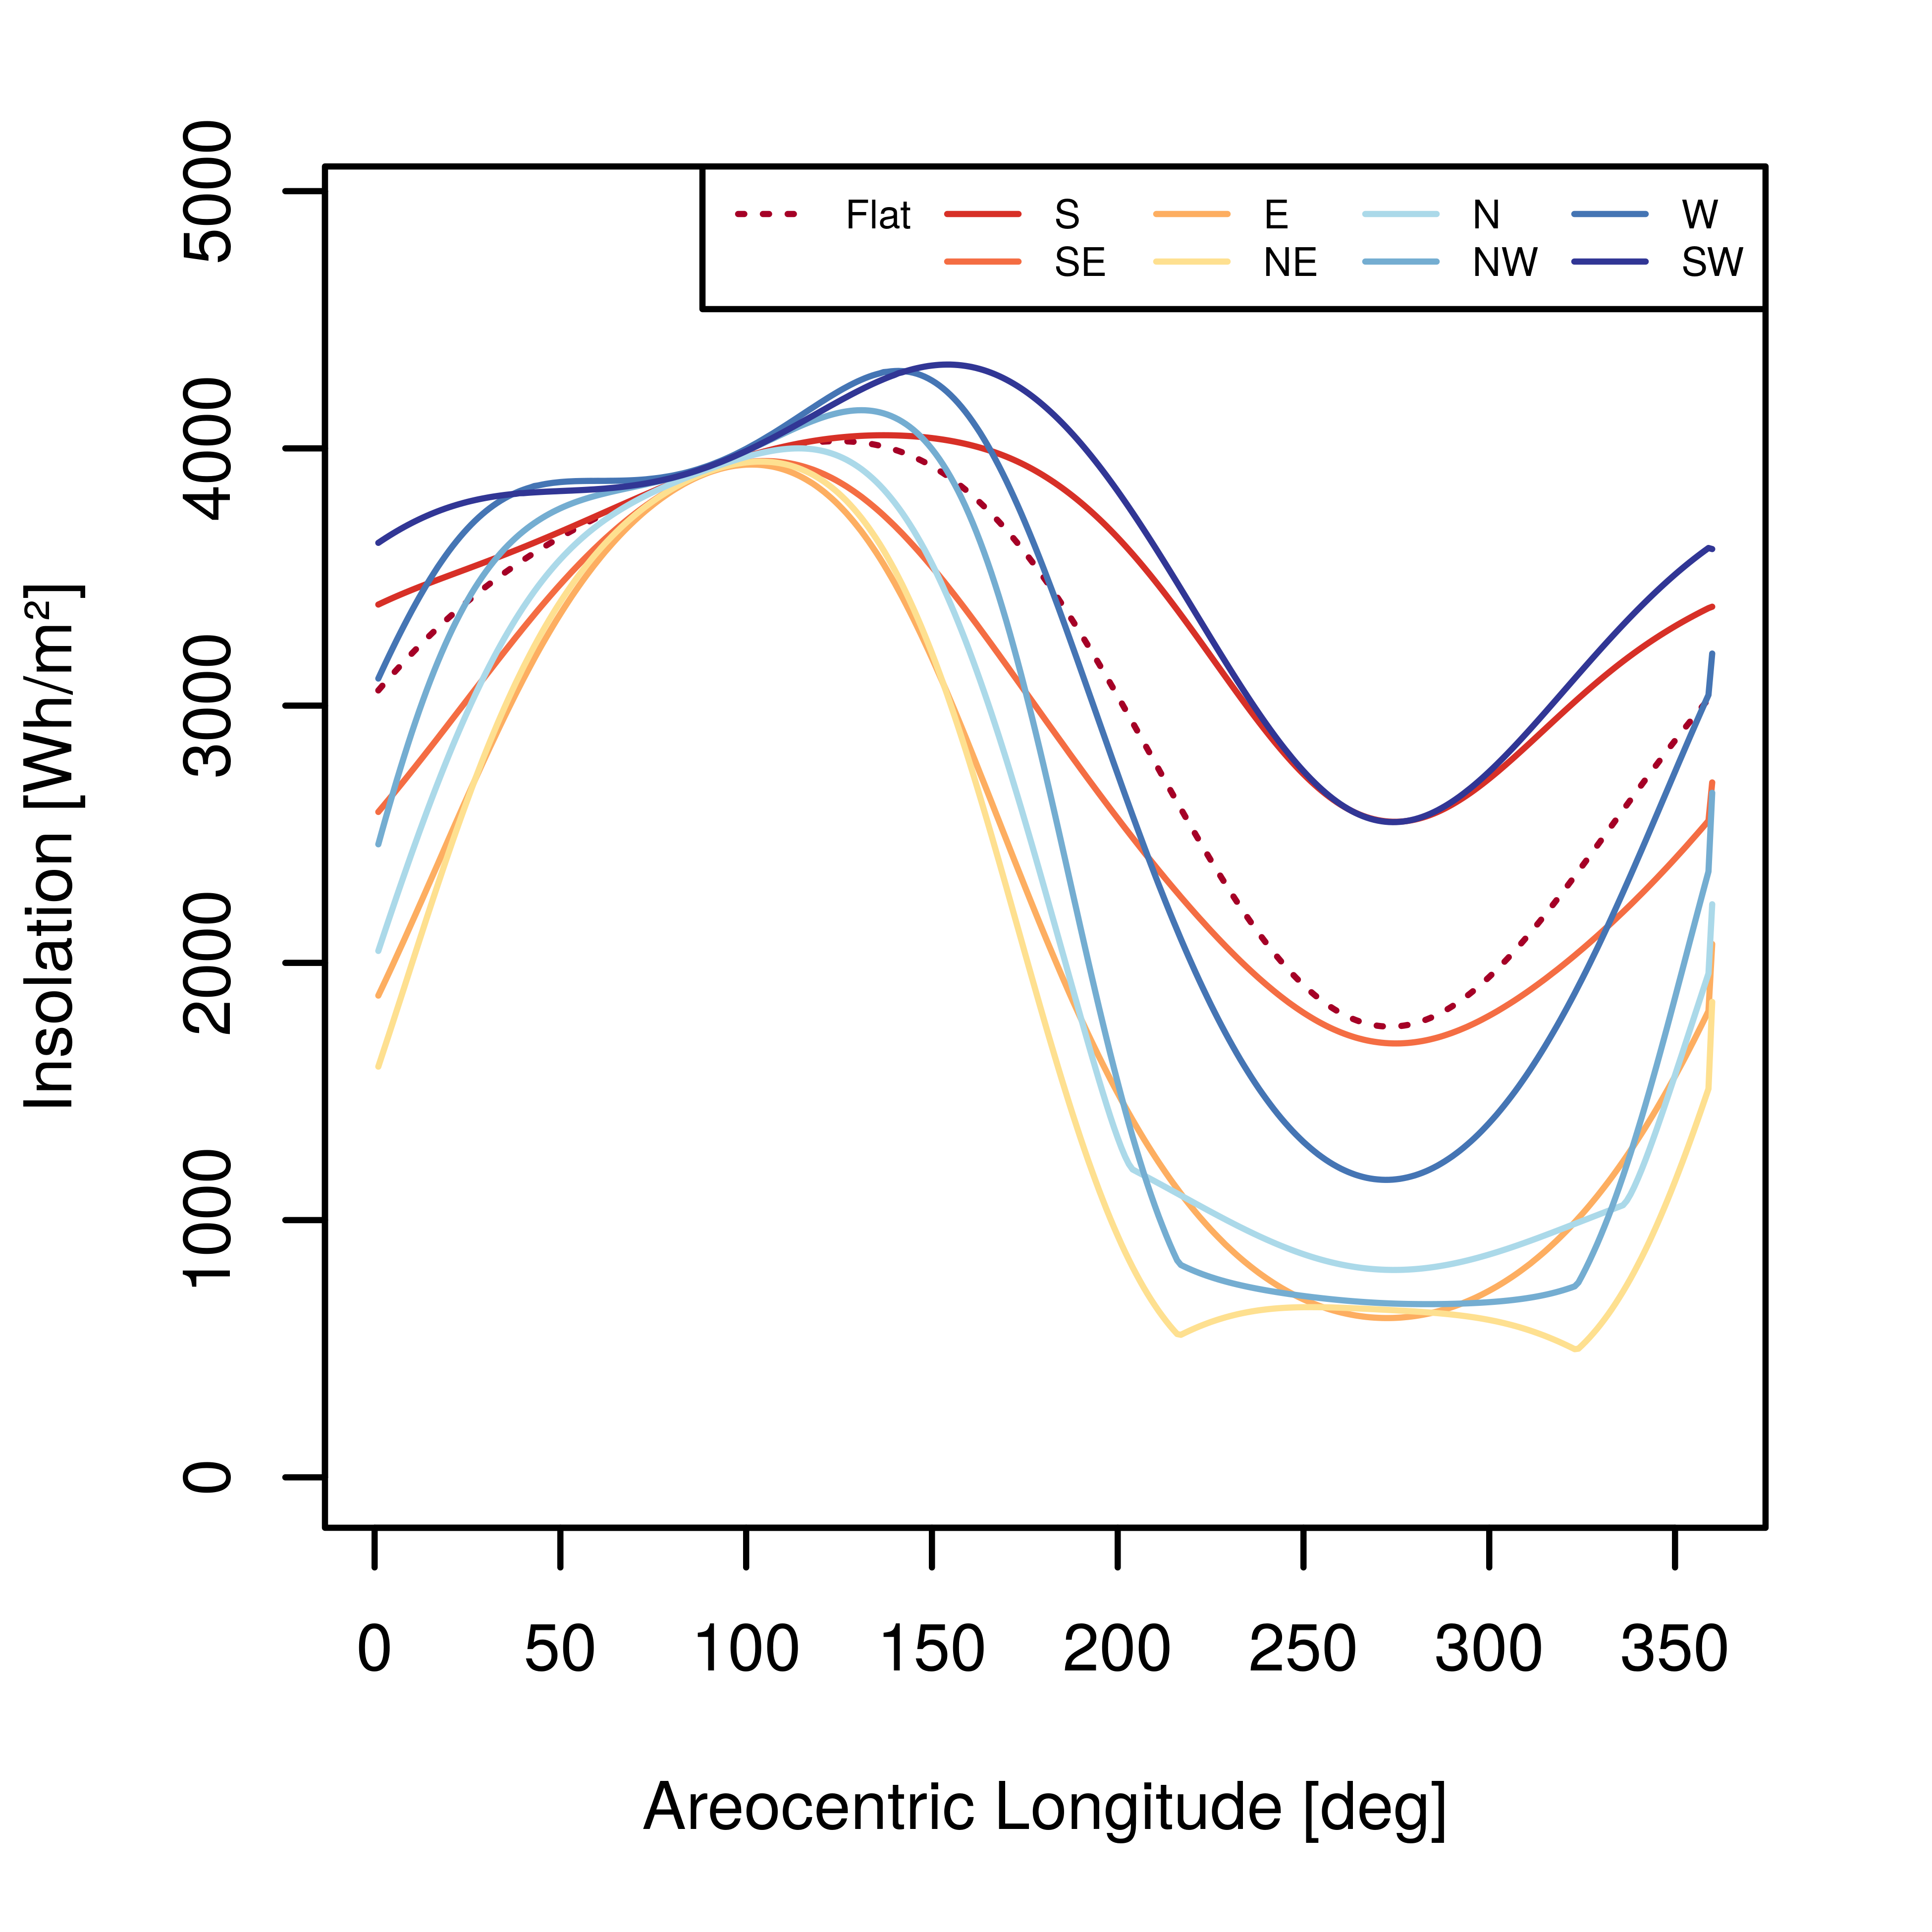
\includegraphics[height=\graphicsHeight]{sections/appendix/optimal-angles/plots/ismenius-cavus-tau-04-and-beta-optimal-based-on-solar-insolation.png}
            \subcaption{Based on the daily beam insolation on the surface from sunrise to sunset}
            \label{fig:sub:optimal-angles-ismenius-cavus-based-on-insolation}
    \end{subfigure}\\[0.8ex]
    \caption[Daily insolation at Ismenius Cavus for optimal inclinations with different orientations]
    {Daily insolation at Ismenius Cavus for optimal inclinations with different orientations. Clear day at $\tau=0.4$. Ismenius Cavus is located in the Northern hemisphere at latitude \SI{34}{\degree}N.}
    \label{fig:plot:optimal-angles-ismenius-cavus}
\vspace{-2ex}
\end{figure}

\section{Conclusion}
The optimal $\beta$ inclination angle is approximated through calculation. However, the assumption that facing the equator is the optimal $\gamma_c$ orientation is not accurate and may instead be at an offset from the direction of the equator depending on latitude and time of year.
